\section{Spanning Forest and Spanning Tree}

A tree $(V,T)$ is a connected graph with no cycles (connected acyclic graph). Every node is reachable from every other node in exactly one way. If $(V,T)$ is connected, then $(V,T)$ is acyclic if and only if $|T| = |V|-1$.

\begin{definition}[Spanning Forest and Spanning Tree] \index{spanning forest} \index{spanning tree}
    Let $G = (V,E)$ be an undirected graph. A spanning forest of $G = (V,E)$ is an acyclic graph $(V,F)$ with $F \subseteq E$. It is a set of tree on disjoint sets of vertices.

    A spanning tree of $G$ is a connected spanning forest of $G$. It contains $|V| - 1$ edges.
\end{definition}

Minimum spanning tree concerns weighted graphs. Consider a weight function $w:\, E \to \R$. A minimum spanning tree is the spanning tree $(V,T)$ of $G$ is a spanning tree of $G$ that minimizes the weight of $T$ where $w(T) = \sum \{ w(e) \mid e \in T \}$.

\section{Computing the Minimum Spanning Tree}

Below is a generic algorithm (template) for finding a minimum spanning tree of a given graph $G=(V,E)$.

\begin{codebox}
    \Procname{$\proc{MST}(G=(V,E),w)$}
    \li $A = \emptyset$
    \li \While $|A| < n-1$ \Do
        \li find an edge $e \in E$ such that there is an MST containing $A \cup \{e\}$ 
        \li $A = A \cup \{e\}$ 
    \li \Return $(V,A)$  
\end{codebox}

The algorithm maintains the loop invariant that there is an MST of $G$ that contains the edges in $A$. On termination, $|A|=n-1$ and then $(V,A)$ is a minimum spanning tree since spanning trees of $G$ have $n-1$ edges.

But then, the question becomes: how to find an edge $e$ that there is an MST containing $A \cup \{e\}$?

$V_1,V_2$ is a partition of $V$ if $V_1 \cup V_2 = V$ and $V_1 \cap V_2 \neq \emptyset$. A \textbf{light edge} crossing the partition is an edge $\{v_1,v_2\} \in E$ with minimum weight such that $v_1 \in V_1$ and $v_2 \in V_2$.
$$
w(\{v_1,v_2\}) = \min \{ w(u_1,u_2) \mid u_1 \in V_1,\, u_2 \in V_2,\, \{ u_1, u_2 \} \in E \}
$$

\begin{theorem} \label{thm:mst-correctness}
    Suppose that $A \subseteq E$ and there is an MST $(V,T)$ of $G$ such that $A \subseteq T$. Let $V_1,V_2$ be a partition such that for all $\{u,v\} \in A$, either $u,v \in V_1$ or $u,v \in V_2$. In other words, no edge in $A$ crosses the partition $V_1$ and $V_2$. Let $e$ be a light edge crossing this partition. Then, there is an MST that contains $A \cup \{e\}$.
\end{theorem}

\begin{proof}
    If $e \in T$, the claim is true. So, suppose $e \not\in T$. Without loss of generality, suppose $e = \{v_1,v_2\}$ where $v_1 \in V_1$ while $v_2 \in V_2$. Since $G $ is connected, there is a simple path $Q$ between $v_1$ and $v_2$ in $T$.

    There is an edge $\{u_1,u_2\}$ on the path $Q$ such that $u_1 \in V_1$ and $u_2 \in V_2$. Note that, by assumption, $\{u_1,u_2\} \not\in A$. Let $Q_1$ be the part of the path $Q$ from $u_1$ to $v_1$, and let $Q_2$ be the part of the path $Q$ from $u_2$ to $v_2$, such that $Q = Q_1 \{v_1,v_2\} Q_2$.

    \begin{center}
        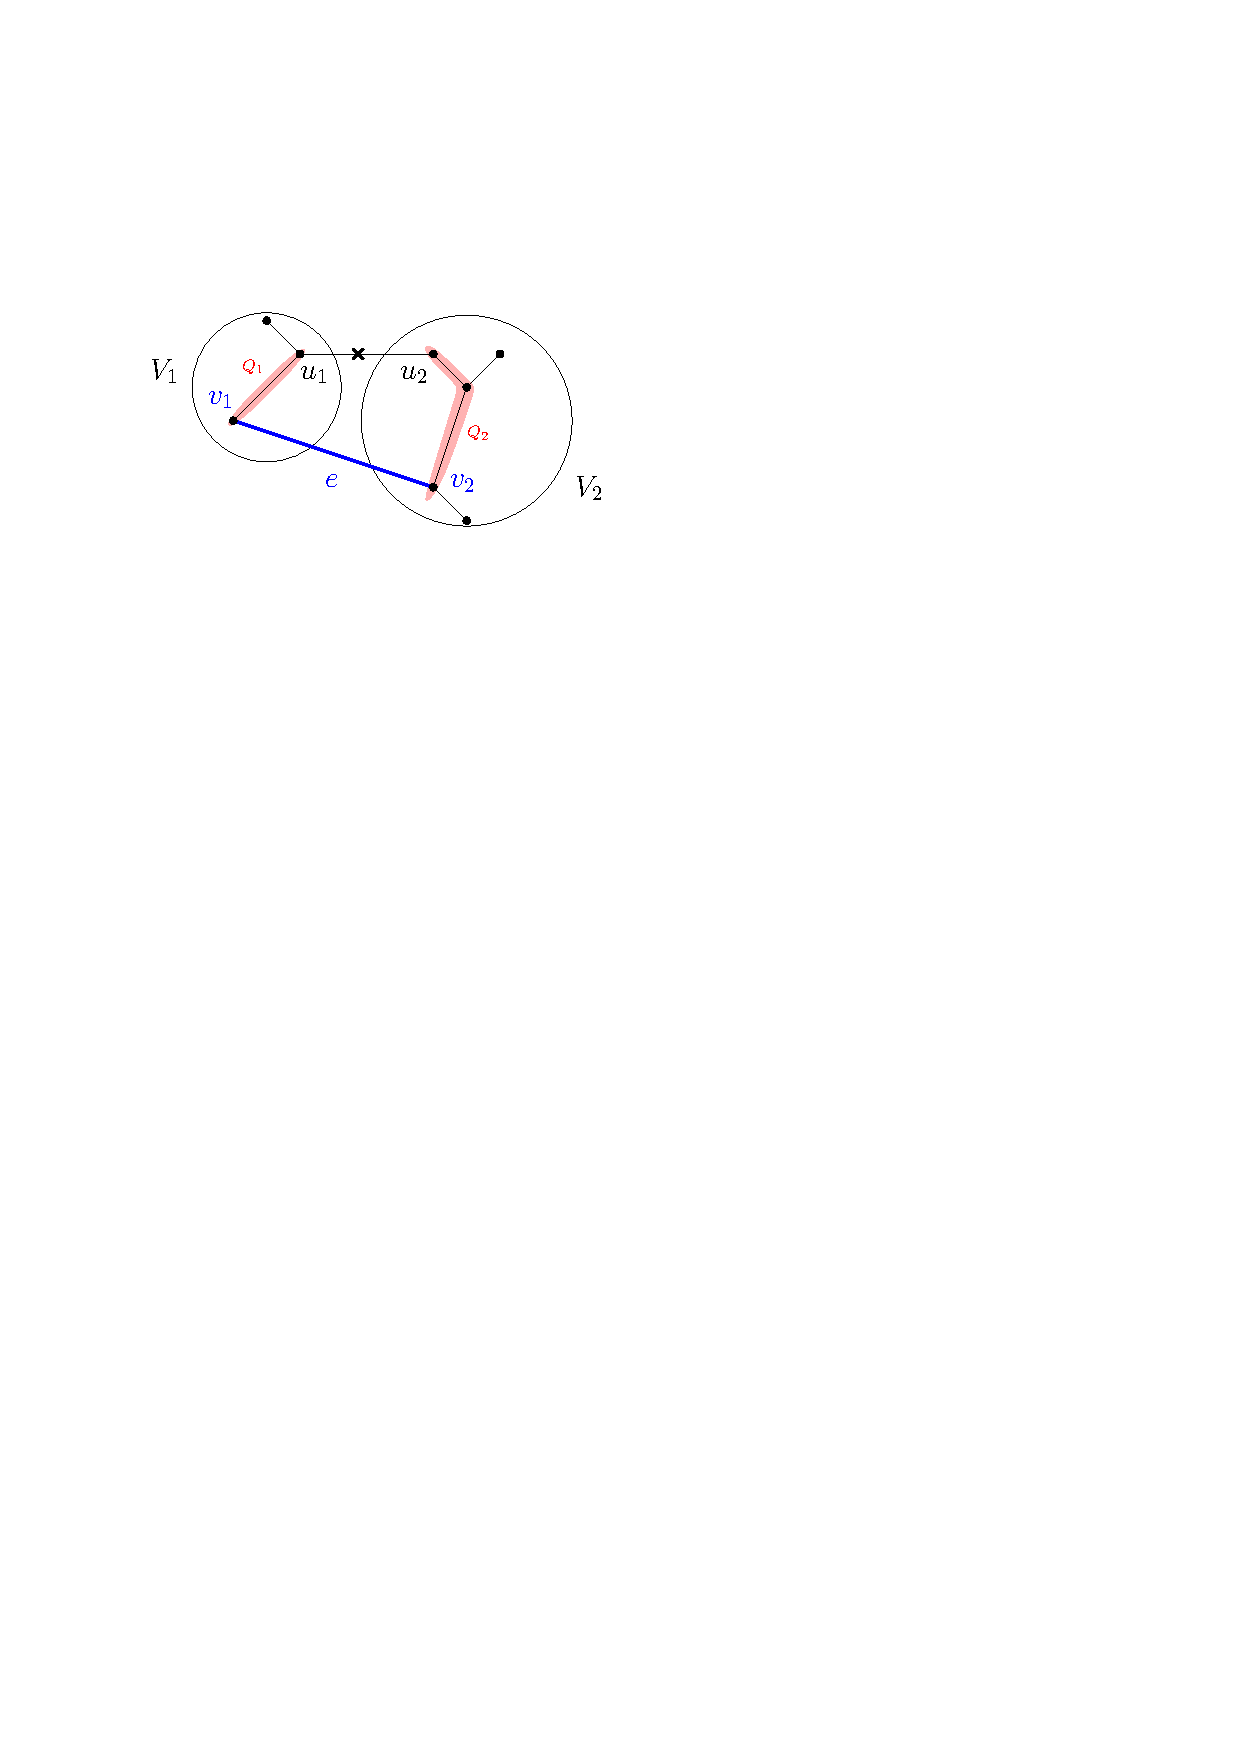
\includegraphics[width=0.5\linewidth]{mst2.pdf}
    \end{center}

    Let $T' = T \cup {e} - \{u_1,u_2\}$. $|T'| = |T| = n-1$ and $A \cup \{\{v_1,v_2\}\} \subseteq T'$.
    
    \textit{Claim}: $(V,T')$ is connected and a tree.

    Let $x,y \in V$. Since $(V,T)$ is connected, there is a path $P$ in $(V,T)$ connecting $x$ and $y$. If $P$ does not contain $\{u_1,u_2\}$ and $u_1$ comes before $u_2$ in $P$. Let $P_1$ be the subpath of $P$ from $x \to u_2$, and let $P_2$ be the subpath of $P$ from $u_2 \to y$ so that $P=P_1 \{u_1,u_2\} P_2$. Then, $P_1,Q_1, \{v_1,v_2\}, Q_2, P_2$ is a path from $x$ to $y$ in $(V,T')$. Hence by generalization, $(V,T')$ is connected. $|T'| = |T| = |V| - 1$ so $(V,T')$ is a tree.

    \textit{Claim}: $w(T') = w(T)$.

    Since $T$ is an minimum spanning tree and $T'$ is a spanning tree,
    $$
    w(T) \leq w(T') = w(T) - w(\{ u_1, u_2 \}) + w(e) \leq w(T)
    $$
    because $w(e) \leq w(\{u_1, u_2 \})$, $e$ is a light edge crossing the partition $V_1,V_2$ and $\{u_1, u_2\}$ crosses the partition. $\{u_1,u_2\} \not\in A$. Hence $T'$ is an MST that contains $A \cup \{e\}$.
\end{proof}

\section{Kruskal's Algorithms}

Invariant: $(V,A)$ is a spanning forest of $G = (V,E)$.

Initially, each vertex is in its own component.
\begin{codebox}
    \Procname{$\proc{Kruskal}(V,A)$}
    \li $A =  \emptyset$
    \li $Q = \proc{Priority-Queue}(\text{all edges $e$ where priority is $w(e)$})$
    \li \For $v \in V$ \Do
        \li $\proc{Make-Set}(v)$
        \End
    \li \While $|A| < n-1$ \Do 
        \li $\{u,v\} = \proc{Extract-Min}(Q)$ 
        \li $u' = \proc{Find-Set}(u)$
        \li $v' = \proc{Find-Set}(v)$
        \li \Comment{if $u$ and $v$ are in different components of $(V,A)$}
        \li \If $u' \neq v'$  \Then
            \li add $\{u,v\}$ to $A$ 
            \li $\proc{Link}(u',v')$
\end{codebox}

Building the priority queue with $m$ elements. This takes $O(m)$ time.

At most $m$ \proc{Extract-Min} operations. This takes $O(m \lg m)$ time.

Alternatively, these two steps can be combined into one step that sorts the edges by weights. If the range of size if $O(m)$, we can use a non-comparison based sorting algorithm like counting sort to achieve an $O(m)$ time bound.

To find connected components, we use disjoint sets. In particular, we have $n$ \proc{Make-Set} operations, at most $2m$ \proc{Find-Set} operations, and $n-1$ \proc{Link} operations. We can use union-by-rank with path compression to implement the disjoint set. The sequence complexity is $O(n + m \log^* n) = O(m \log^*n)$ where $n \leq m$. Alterenatively, we can use linked lists with union-by-size, which takes $O(m + n \log n)$. But no matter what implementation we use for the disjoint set, we still have the $O(m \log m)$ overhead from the heap/sorting.

\begin{figure}
    \centering
    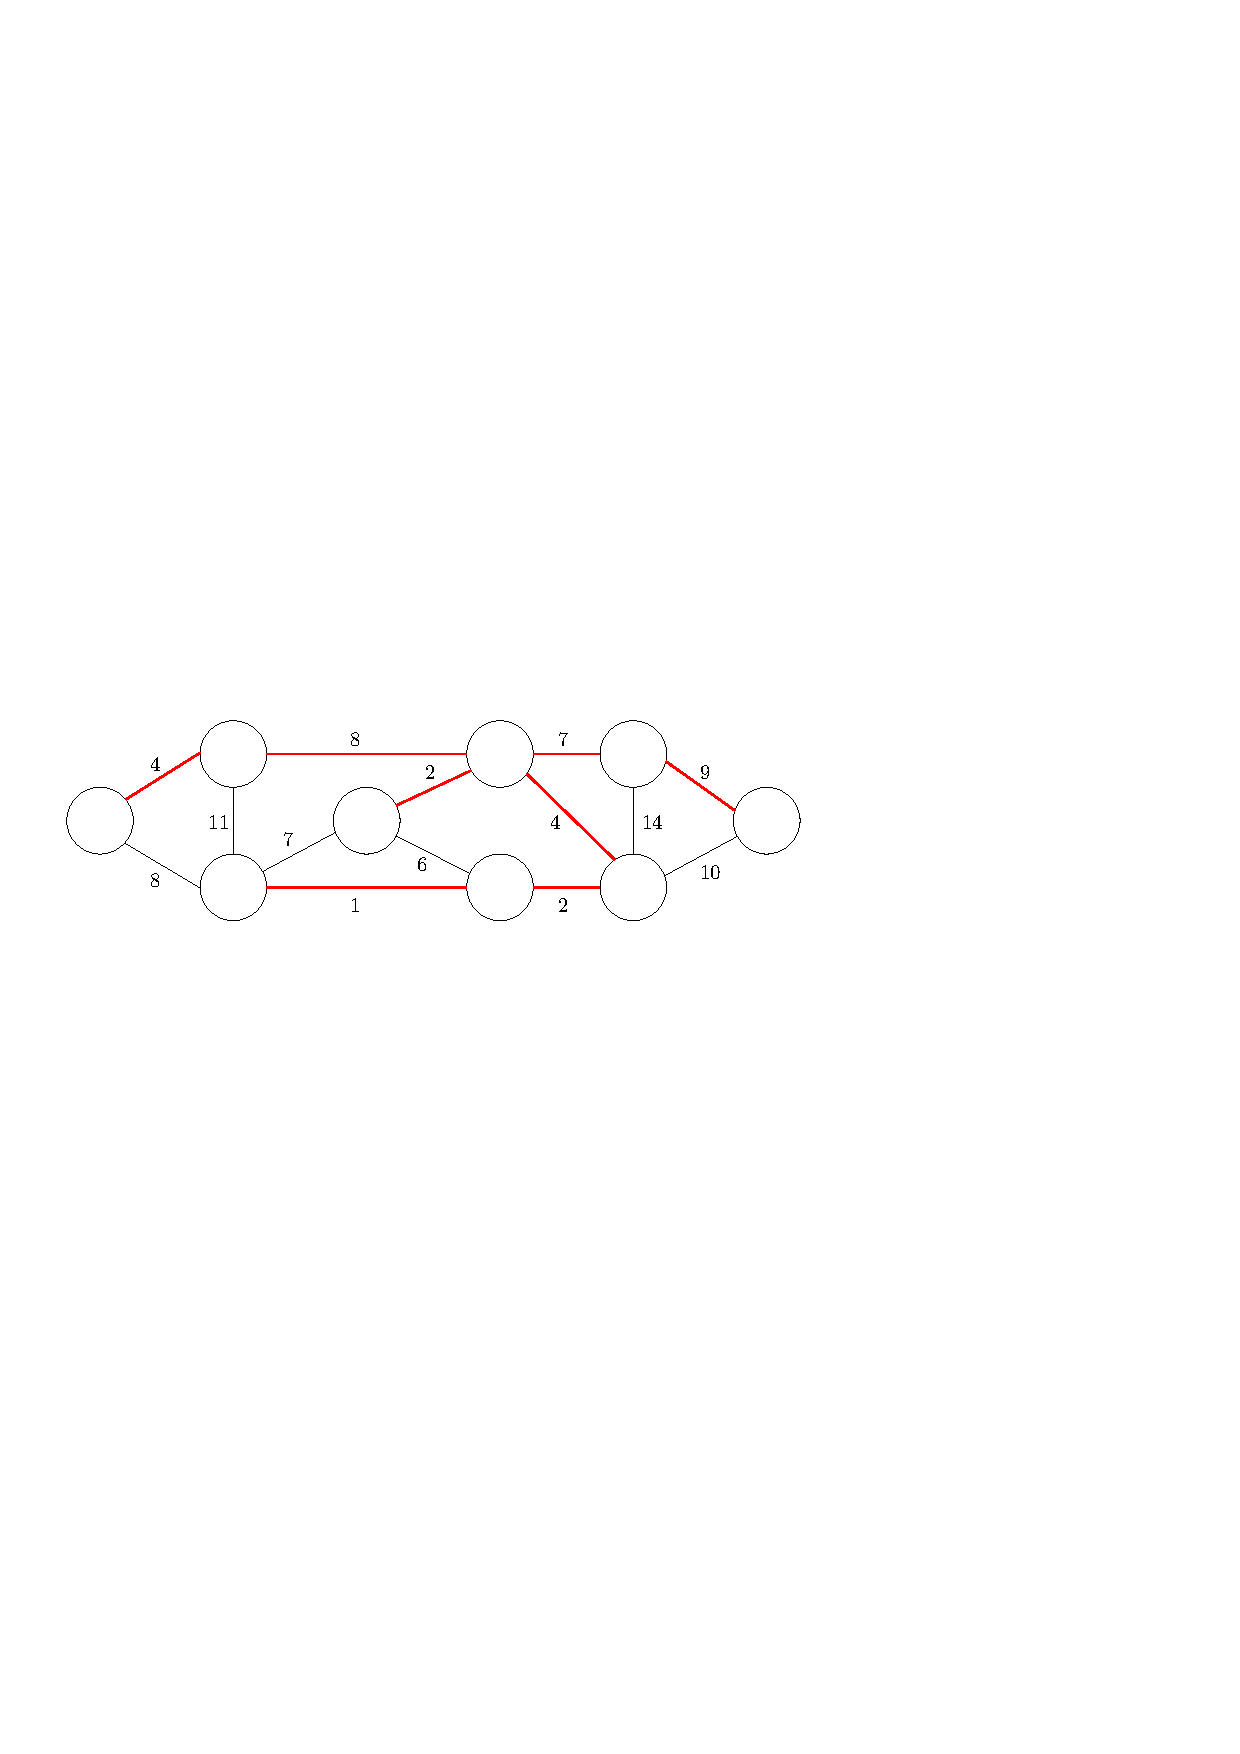
\includegraphics[width=0.8\linewidth]{mst/kruskal.pdf}
    \caption{The minimum spaning tree resulted from running the Kruskal's algorithm. A step-by-step diagram can be found at pp 632 of CLRS.}
\end{figure}


\section{Prim's Algorithm}

The idea is to grow the MST from a single vertex $r$. $V'$ is the set of nodes reachable from $r$ via edges in $A$. We maintain the invariant that $(V',A)$ is a tree.

Repeatedly add a light edge crossing the partition $(V',V-V')$ to $A$.

\begin{codebox}
    \Procname{$\proc{Prim}(V,r)$}
    \li \For $v \in V - \{r\}$ \Do
        \li $\attrib{v}{priority} = \infty$
        \li $\attrib{v}{parent} = \const{nil}$ \End
    \li $Q = \proc{Priority-Queue}(V-\{r\})$
    \li $u = r$ 
    \li \While $Q \neq \emptyset$ \Do
        \li \For neighbor $v$ of $u$ \Do
            \li \If $v \in Q$ \textbf{and} $w(\{u,v\}) < \attrib{v}{priority}$ \Then
                \li $\attrib{v}{priority} = w(\{u,v\})$
                \li $\proc{Decreae-Priority}(Q,v,\, \id{priority}=w(\{u,v\}))$ 
                \li $\attrib{v}{parent} = u$ \End
            \End
        \li $u = \proc{Extract-Min}(Q)$
        \li add $\{u,\attrib{u}{parent}\}$ to $A$
        \End
    \li \Return $(V,A)$ 
\end{codebox}

\begin{figure}
    \centering
    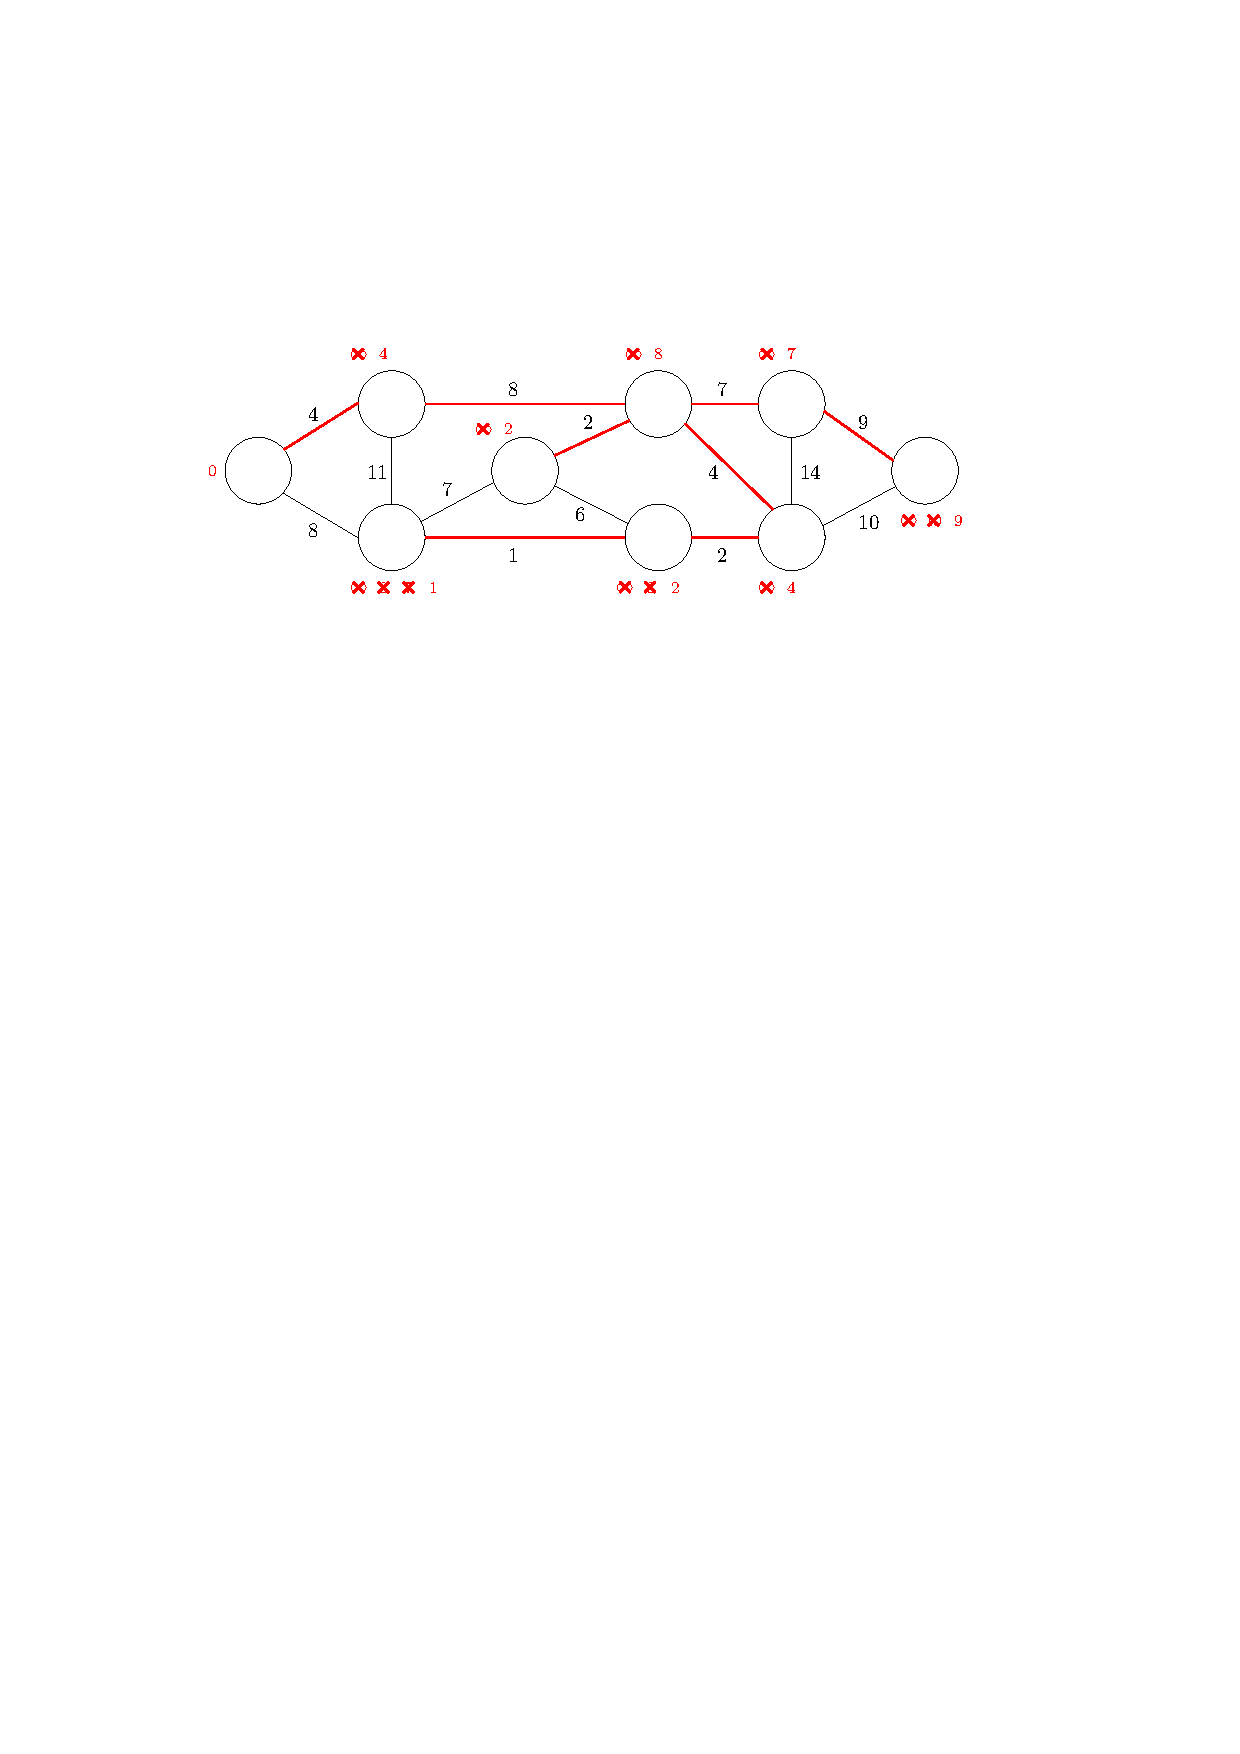
\includegraphics[width=0.8\linewidth]{mst/prim.pdf}
    \caption{The minimum spaning tree resulted from running the Prim's algorithm. The priorities are labeled in red next to each node.}
\end{figure}

Building the priority queue takes $\Theta(n)$ time. There are another $(n-1)$ \proc{Extract-Min} operations, and $m$ decrease priority operations. We can augment vertices so we know whether they are in $Q$ or in $V'$ with $O(1)$ per lookup.

If we implement the priority queue using a heap, both \proc{Extract-Min} and decreasing priority are $O(\log n)$. If we use a Fibonacci heap, it takes $O(1)$ amortized for each \proc{Decrease-Priority} operation, and \proc{Extract-Min} still takes $O(\log n)$. Overall, the algorithm requires $O(m + n \log n)$  using a Fibonacci heap.

Both Kruskal and Prim's algorithms are greedy algorithms. At each step/iteration, it takes the locally optimal step. At each step of the algorithm, one of several possible choices must be made. In the context of finding the MST, the choices involve what edge to add to $A$. A greedy strategy chooses the edge which is best at the moment (locally optimal).

In Kruskal's algorithm, the choice is the edge of smallest weight that connects 2 different components. In Prim's algorithm, the choice is the edge of smallest weight that connects a vertex in $V-V'$ to a vertex in $V-V'$. The partition $V'$ starts as a single node and grows to span all nodes in the graph.

By Theorem \ref{thm:mst-correctness}, both Kruskal's and Prim's algorithms guarantee that the result is a globally optimal minimum spanning tree. In general, greedy algorithms do not guarantee a globally optimal solution, but they often provide a good approximation to many hard-to-solve problems.